\section{\esp Introdução}

Atualmente a aplicação de grafos é cada vez mais importante para o mundo dos algoritmos e estrutura de dados, por ser ótimo para a resolução de problemas. Um dos problemas dos grafos é o custo que tem-se para aplicar alguns algoritmos em grafos muito grandes em quantidade de vértices (V) e arestas (E). Por isso o trabalho tem como intuito, abordar o tempo de execução da identificação de um caminho euleriano em um grafo aleatório de 100, 1000, 10000 e 100000 vértices, juntamente com a estratégia de identificação de pontes feitas pelo algoritmo Naive e \cite{tarjan}, que serão utilizados no algoritmo Fleury para a escolha das arestas corretas. 

\section{\esp Desenvolvimento}
O projeto foi desenvolvido em Python (CPython), a qual é uma linguagem interpretada, devido isso o tempo de execução de alguns algoritmos pode demorar mais que as outras linguagens, como mostrado na figura \ref{fig:figure1}, o objetivo de utilizar Python foi ter a possibilidade de ter uma comparação com os demais trabalhos em tempo de execução dos algoritmos.

\begin{figure}[ht]
    \centering
    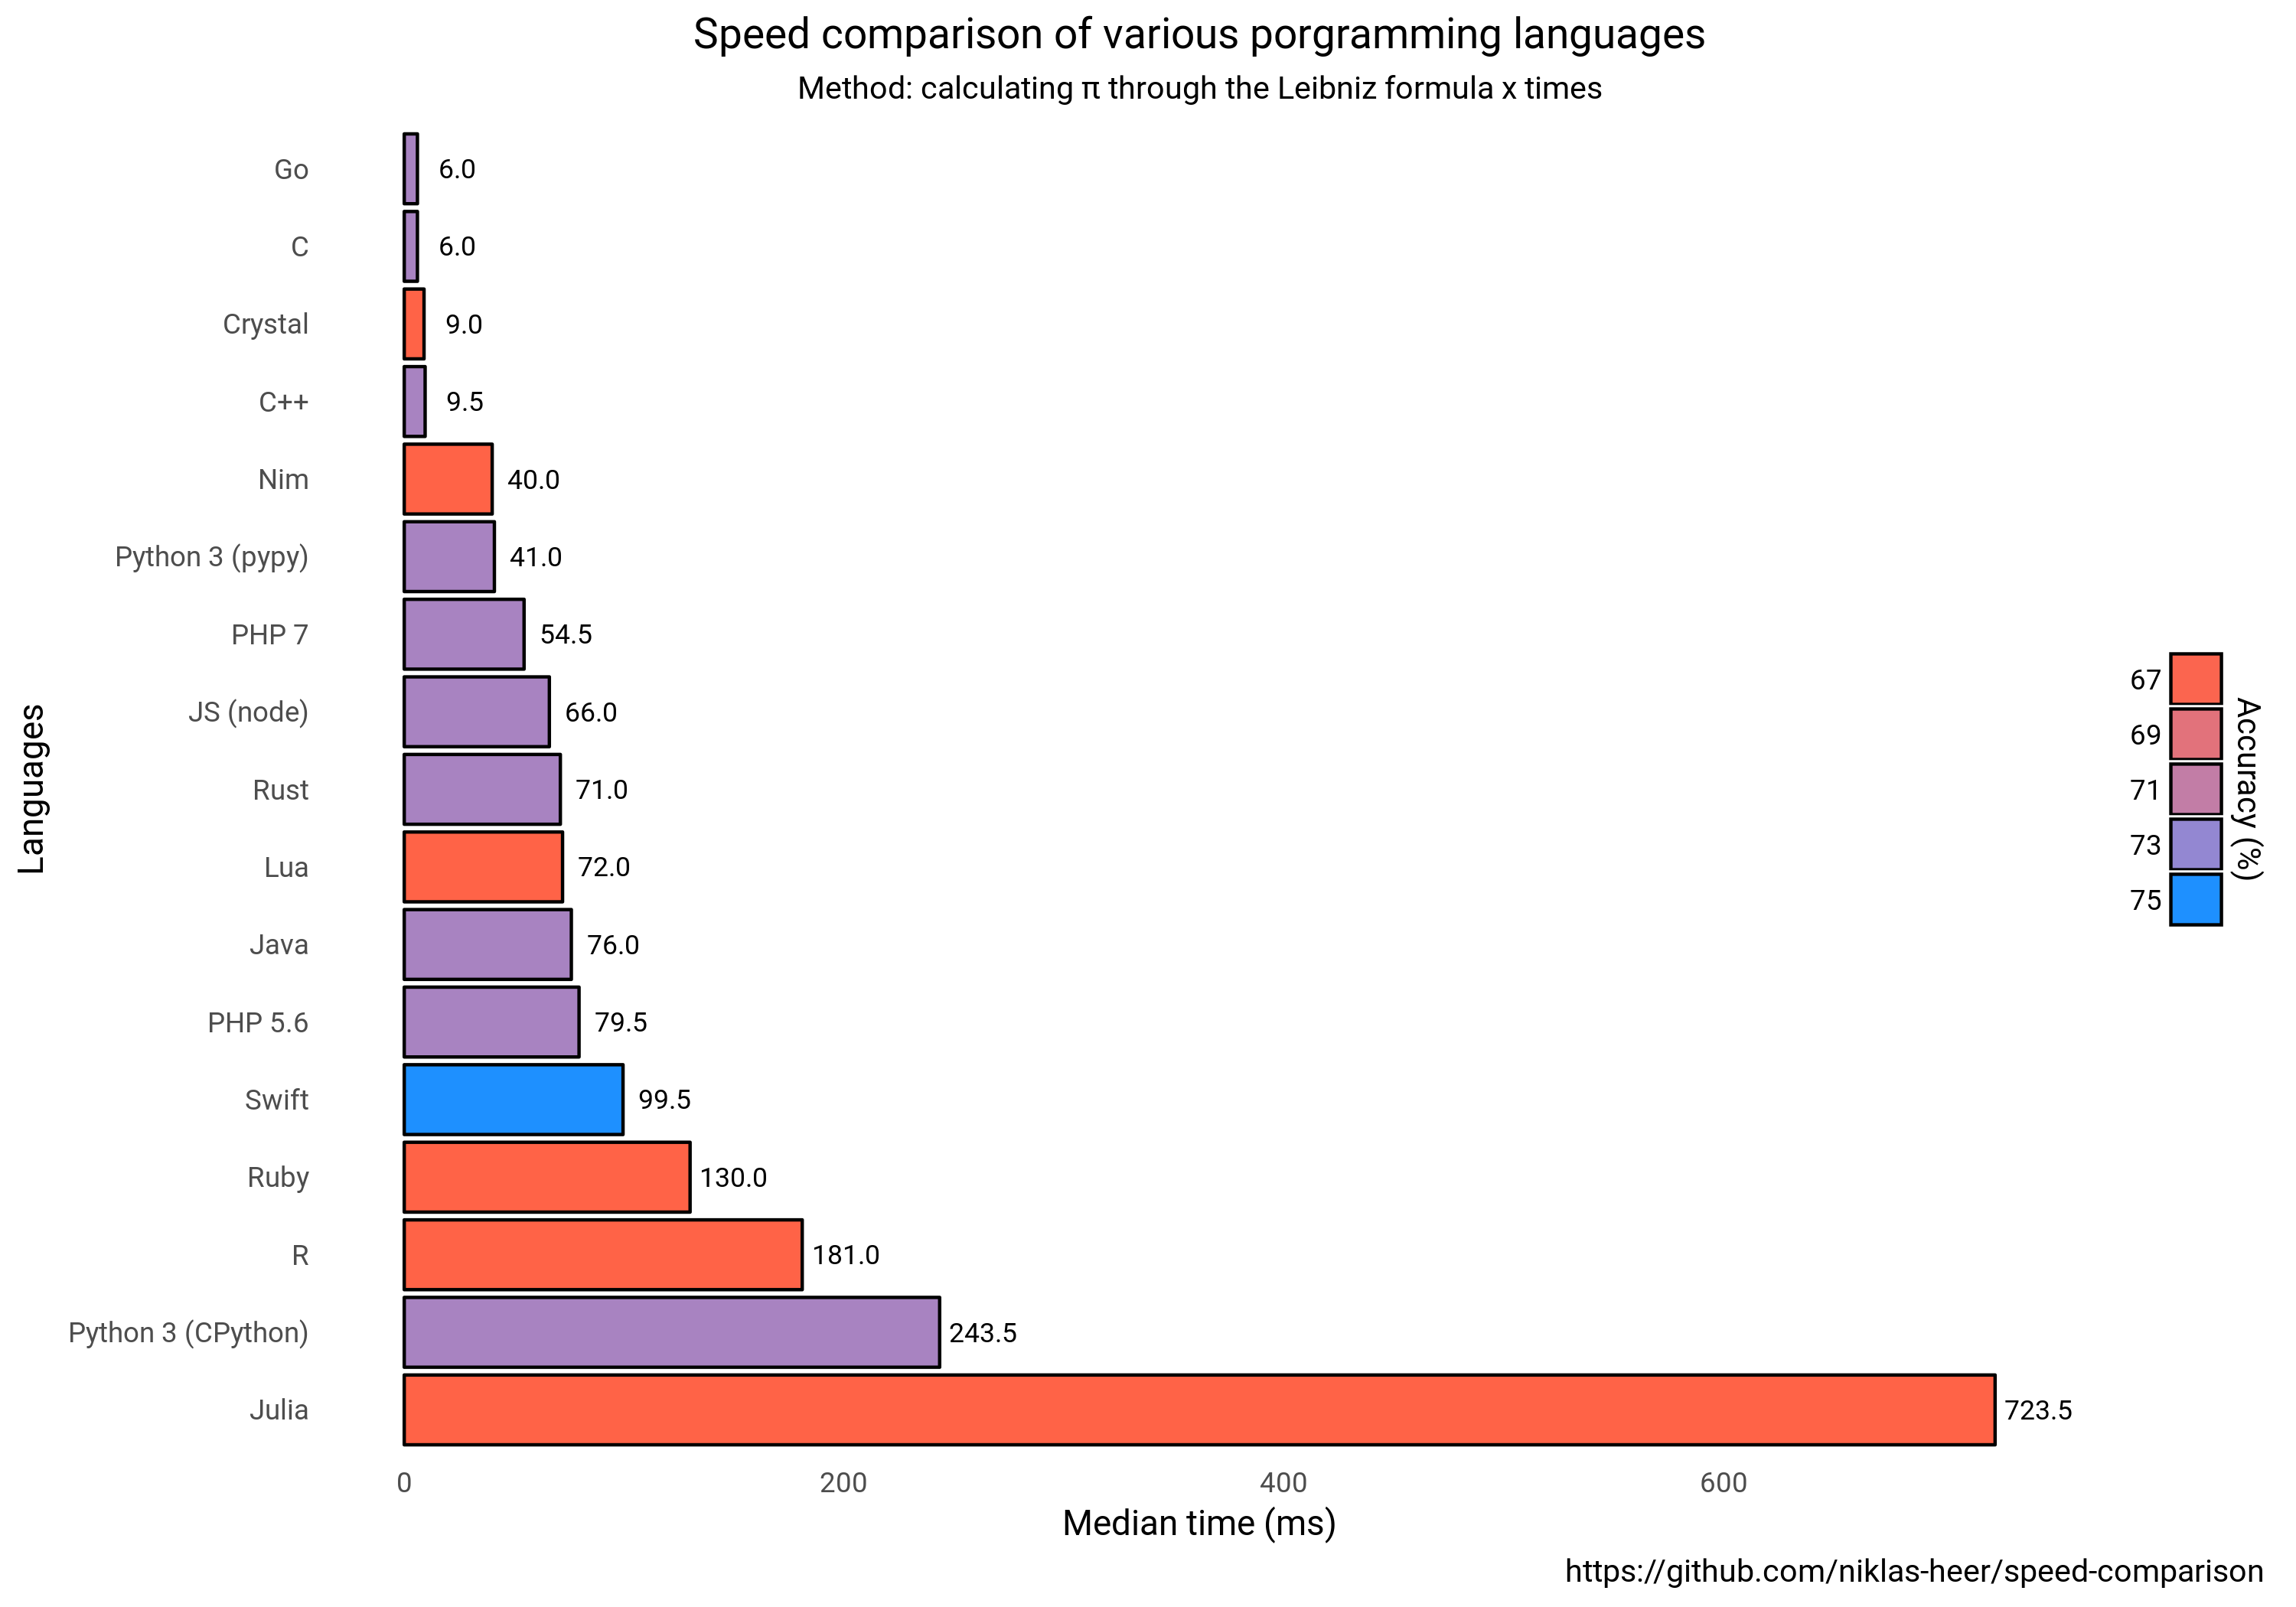
\includegraphics[width=.9\textwidth]{figuras/speed-comparision-programming.png}
    \caption{Comparação de velocidade entre as linguagens}
    \label{fig:figure1}
\end{figure}

\subsection{\esp Criação dos grafos aleatórios}
\subsubsection{\esp Grafo euleriano}
Um grafo euleriano é um grafo onde todos os seus vértices possuem grau par. Com isso, basta aplicar um algoritmo que ligue o vértice (i) no vértice (i + 1). Com isso o grafo será cíclico e todos seus vértices serão de grau 2, como mostrado na figura \ref{fig:figure2}.

\begin{figure}[ht]
    \centering
    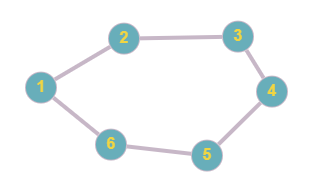
\includegraphics[width=.2\textwidth]{figuras/eureliano.png}
    \caption{Grafo euleriano}
    \label{fig:figure2}
\end{figure}

\subsubsection{\esp Grafo semi-euleriano}
Um grafo semi-euleriano é um grafo onde onde tem apenas dois vértices de grau ímpar. Com isso, para criar um grafo aleatório semi-euleriano bastava criar um grafo euleriano e sortear uma aresta para incidir em dois vértices, transformando o grau de 2 vértices do grafo para 3, como mostrado na figura \ref{fig:figure3}.

\begin{figure}[ht]
    \centering
    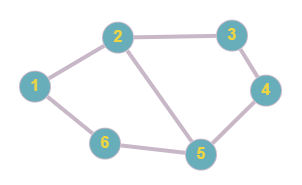
\includegraphics[width=.2\textwidth]{figuras/semi-eureliano.png}
    \caption{Grafo semi-euleriano}
    \label{fig:figure3}
\end{figure}

\subsubsection{\esp Grafo não euleriano}
Um grafo não euleriano é um grafo onde onde tem mais de dois vértices de grau ímpar. Com isso, para criar um grafo aleatório não euleriano foi necessário criar apenas um grafo eureliano e sortear duas arestas no grafo, sem repeti-lás, para que assim o grafo tenho 4 vértices de grau ímpar, tornando assim o grafo em não eureliano, como exemplificado na figura \ref{fig:figure4}.

\begin{figure}[ht]
    \centering
    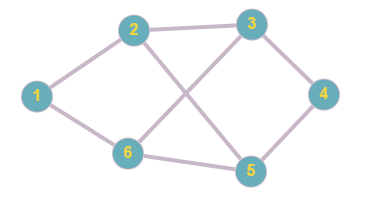
\includegraphics[width=.2\textwidth]{figuras/not_eurelian.png}
    \caption{Grafo não euleriano}
    \label{fig:figure4}
\end{figure}

\subsection{\esp Caminho euleriano - Fleury}
Para implementação do algoritmo Fleury no qual consiste em buscar um caminho euleriano seja ele fechado ou aberto em um grafo, caso o grafo não seja eureliano ou semi-eureliano ele não vai conter um caminho euleriano, foi utilizado o material disponibilizado pelo Prof. Zenilton no Canvas, ferramenta de organização de materias da faculdade, mostrando na \ref{fig:figure5}, onde pode-se usar como referência para implementar na linguagem Python:

\begin{figure}[ht]
    \centering
    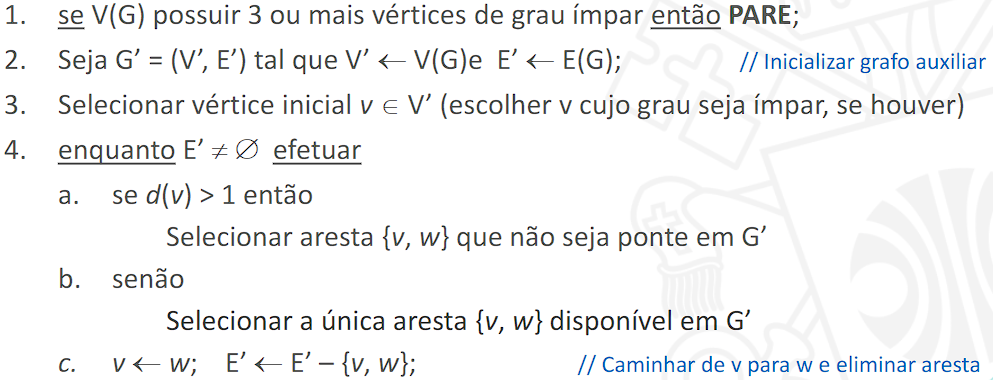
\includegraphics[width=.9\textwidth]{figuras/fleury.png}
    \caption{Algoritmo Fleury - Prof. Zenilton}
    \label{fig:figure5}
\end{figure}

\subsubsection{\esp Identificação pontes - Naive}
O algoritmo Naive faz uma busca muito custosa pelas pontes, já que ele percorre todos os vértices do grafo fazendo às seguintes operações: remove uma aresta da lista de adjacência do grafo, após isso faz uma busca em largura. Visto que, para cada vértice existente no grafo, ele deve ser visitado uma única vez e para cada aresta existente, ela também deve ser visitada uma única vez, para conferir se o grafo é conexo, onde se todos vértices forem visitados o grafo é conexo, caso contrário não é conexo, como mostrado na figura \ref{fig:figure6} de forma visual. Com isso, o algoritmo tem o custo de complexidade \textbf{O(E * (V + E))}.

\newpage
\begin{figure}[ht]
    \centering
    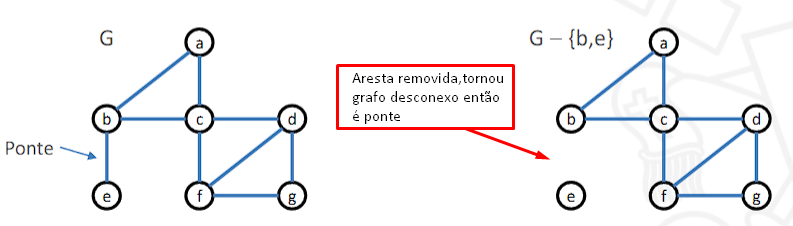
\includegraphics[width=.9\textwidth]{figuras/naive.png}
    \caption{Identificação pontes (Naive) - Prof. Zenilton}
    \label{fig:figure6}
\end{figure}

\subsubsection{\esp Identificação pontes - Tarjan}
Para implementação do algoritmo Tarjan foi utilizado da ideia do seguinte algoritmo retirado do artigo \cite{tarjan}, a ideia da implementação pode ser mostrada na figura \ref{fig:figure9}, onde o algoritmo consiste em achar uma árvore de abrângencia \cite{spanning} utilizando o algoritmo de busca em profundidade, onde pode ser encontrado em tempo linear, onde começando a partir de um vértice arbitrário v , percorrendo os vizinhos dos vértices descobertos. Aplicando-se assim, um tempo para as variavéis \textbf{LOW[]} e \textbf{DISC[]}, sempre considerando o grafo como conexo com apenas 1 componente, tendo em vista isso, após a seguinte condição \textbf{disc[u] < low[v]} ter sido verdadeira durante a busca em profundidade a aresta \textbf{[u, v]} é uma ponte. Com isso, o artigo trata que o algoritmo possui uma complexidade \textbf{O(V + E)}, muito menos custoso.

\begin{figure}[ht]
    \centering
    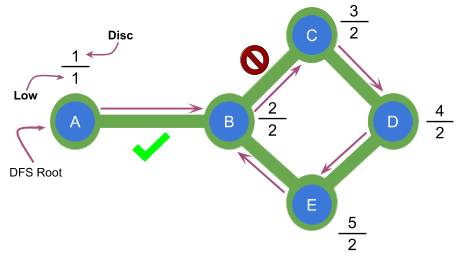
\includegraphics[width=.8\textwidth]{figuras/tarjan_1974.png}
    \caption{Tarjan \cite{tarjan_code}}
    \label{fig:figure9}
\end{figure}

\newpage
\section{\esp Analise de resultados}

Todos os experimentos foram realizados em uma máquina: 
\begin{itemize}
  \item Processador i7-11390H - 3.4GHz - 2918Mhz - 4 núcleos 
  \item Memória - 16GB - DDR4 - 3200MHz
  \item Windows 11
  \item SSD 500GB
\end{itemize}


\subsection{\esp Tabelas}

A tabela \ref{tab:tabela1} mostra todos os tempos de execução dos algoritmos Naive, o qual é um algoritmo mais custoso. Porém a tabela \ref{tab:tabela2} possui todos os resultados da utilização algoritmo de Tarjan desenvolvido em 1974, onde o próprio autor aborda no artigo \cite{tarjan} que trata de um algoritmo de busca de pontes de forma mais eficiente. Vale resaltar que na tabela \ref{tab:tabela1} alguns resultados foram escondidos com NA, pelo tempo de execução ser muito demorado, mais de 8 horas, sem obter resultado, além dos testes terem sido realizados com pelo menos 5 grafos para cada tipo de grafo, para se obter uma média do tempo estimado para execução do algoritmo. Com isso, a cada execução de uma aresta no algoritmo Fleury foi buscado as pontes após a remoção, fazendo com que o tempo do algoritmo Fleury seja mais demorado, por isso a baixo aborda o tempo médio de busca de pontes em vários grafos aleatórios gerados por código.

% Tabela
\begin{table}[htb]
	\centering
	\caption{\hspace{0.1cm} Algoritmo Naive}
	\vspace{-0.3cm} % espaço entre titulo e tabela
	\label{tab:tabela1}
	% Conteúdo da tabela
	\begin{tabular}{l|c|c}
  \hline
    \textbf{Vértices}	& \textbf{Grafo} & \textbf{Tempo (segundos)} \\
    \hline
     100	 & Euleriano      &  0000.0039     \\
     1000	 & Euleriano      &  0000.4889     \\
     10000	 & Euleriano      &  0127.1838   \\
     100000  & Euleriano      &  NA         \\
     100	 & Semi-euleriano &  0000.0159     \\
     1000	 & Semi-euleriano &  0001.2655     \\
     10000	 & Semi-euleriano &  0515.5800   \\
     100000  & Semi-euleriano &  NA         \\
     100	 & Não-euleriano  &  0000.0334     \\
     1000	 & Não-euleriano  &  0003.5124     \\
     10000	 & Não-euleriano  &  3680.2427  \\
     100000  & Não-euleriano  &  NA         \\

     \hline
 \end{tabular}
 	\vspace{.1cm}  %espaço entre tabela e fonte
	\small
	% Fonte
	{\footnotesize\\ GitHub - zTrolly}
\end{table}

% Tabela
\newpage
\begin{table}[htb]
	\centering
	\caption{\hspace{0.1cm} Algoritmo Tarjan 1974}
	\vspace{-0.3cm} % espaço entre titulo e tabela
	\label{tab:tabela2}
	% Conteúdo da tabela
	\begin{tabular}{l|c|c}
  \hline
    \textbf{Vértices}	& \textbf{Grafo} & \textbf{Tempo (segundos)} \\
    \hline
     100	 & Euleriano      &  0000.0007  \\
     1000	 & Euleriano      &  0000.0400  \\
     10000	 & Euleriano      &  0003.4584  \\
     100000  & Euleriano      &  0383.9894  \\
     100	 & Semi-euleriano &  0000.0007  \\
     1000	 & Semi-euleriano &  0000.0484  \\
     10000	 & Semi-euleriano &  0007.9425  \\
     100000  & Semi-euleriano &  0765.4123  \\
     100	 & Não-euleriano  &  0000.0009  \\
     1000	 & Não-euleriano  &  0000.0548  \\
     10000	 & Não-euleriano  &  0050.2345  \\
     100000  & Não-euleriano  &  4896.9488  \\

     \hline
 \end{tabular}
 	\vspace{.1cm}  %espaço entre tabela e fonte
	\small
	% Fonte
	{\footnotesize\\ GitHub - zTrolly}
\end{table}

\subsection{\esp Discussão dos resultados}
\subsubsection{Algoritmo Naive}
A partir dos resultados obtidos através da execução dos algoritmos, pode-se observar que o algoritmo do Naive é muito mais custoso que o algoritmo do Tarjan, como pode ser explicado na figura \ref{fig:figure7}, onde o algoritmo está no intervalo vermelho, fazendo com que o tempo de execução no eixo Y aumente conforme o número de arestas e vértices, mostrando que pelo algoritmo Naive apresentar diversas operações nas arestas e nos vértices, fazendo assim que a complexidade faça passar pelas arestas várias vezes, tendo um custo de complexidade muito alto, sendo ele O(E * (V + E)), isso explica o tempo elevado que execução, dependendo da quantidade de arestas e vértices que um grafo possui.

\subsubsection{Algoritmo Tarjan}
O algoritmo do Tarjan é menos custoso, pois ele apresenta soluções que fazem diminuir consideravelmente o acesso as arestas, ou seja, o algoritmo evitou que as arestas precisassem ser visitadas mais de uma vez, fazendo assim que o custo seja linear ao aumento do números de vértices e arestas como mostrado na figura \ref{fig:figure7}, ou seja, o algoritmo estaria no intervalo verde, onde ele passa por todas as arestas, mostrando assim que a complexidade do algoritmo é O(V + E).

\newpage

\begin{figure}[ht]
    \centering
    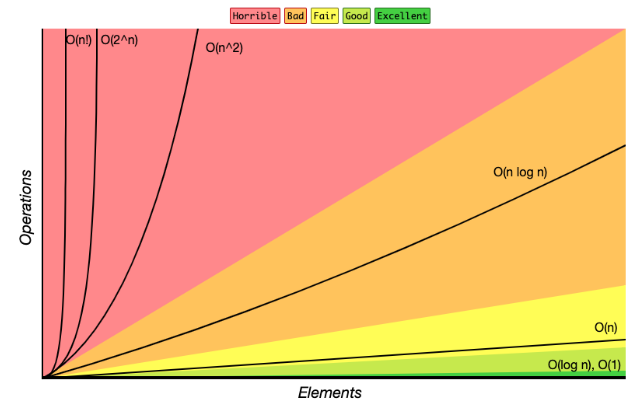
\includegraphics[width=.8\textwidth]{figuras/complexidade.png}
    \caption{Gráfico Complexidade}
    \label{fig:figure7}
\end{figure}

\section{\esp Conclusão}
Pode-se concluir então que caso seja necessário implementar um algoritmo de identificação de pontes, por questão de tempo de execução o algoritmo de Tarjan é mais viável, por mais que seja de maior complexidade de implementação, já o algoritmo Naive é de mais fácil implementação, porém o custo de se ter uma fácil implementação vem no tempo, onde ele gasta um tempo longo para encontrar as pontes de grafos com muitos vértices e arestas.